\chapter{Methods}\label{chap:methods}

As we reviewed in Chapter \ref{chap:introduction}, so far the problem of IO and especially on 3D datasets is largely unexplored.
In this project we study several approaches at DL using inertial datasets for the task of IO.
Some of these approaches are inspired from the existing literature, and some of them are original of this work.
In this second chapter, we will discuss the different DL training pipelines that we studied and trained, and what knowledge we got from their results.
The aim of this section is to provide logically structured information about our findings during our  iterative succession of experiments and discoveries.
We will therefore be making special focus on the mathematical reasoning behind our decisions, and how each one is followed by the next generation of deep models.
As such, some results of these experiments will be provided in this chapter whenever they are useful to justify a decision, but Chapter \ref{chap:experiments} will be the one focused on this purpose.

As we showed during the state-of-the-art review in Section \ref{sec:related_work}, there is still no standardized pipeline on how to work with windows of inertial data. 
By far, the two most used approaches were CNN's and LSTM's but, to the best of our knowledge, none of the studies managed to proof that one was rigorously better than the other. 
Only \cite{DBLP:journals/corr/abs-1802-02209} did an empirical comparison between both, and in their results it was only shown that LSTM-based architectures were training faster (in terms of loss function reduction per epoch), but really no specifications about the CNN architectures were provided.

Because of this, and since it was is also the simplest of all the studied approaches, we begin by reproducing and adapting the work of \cite{DBLP:journals/corr/abs-1808-03485}, described in Section \ref{sec:speed_reg}. 

\section{First model: CNN speed regressor}

Another reason why we decide to start working with CNN's, is that they train much faster than RNN's, since for the latter the hidden state sequences cannot be computed in parallel. 
We transcribe the CNN model from the open source Torch code in \cite{DBLP:journals/corr/abs-1808-03485} to Tensorflow 2.0a, and train it using windows of 200 samples of IMU data, as described in the original article. 
To increase the amount of training data and to enforce shift-invariant feature extractions, we use an overlap of $w-1$ in between two windows of data (i.e., we generate one new training sample for each IMU recording, so that all the previous samples are shifted by one position in time).

We also modify the original structure shown in Figure \ref{fig:speed_net} of the model by adding a MaxPooling layer between the convolution block and the dense block (even though in the paper they explicitly specify that they didn't use them).
\begin{figure}[h]
   \centering
   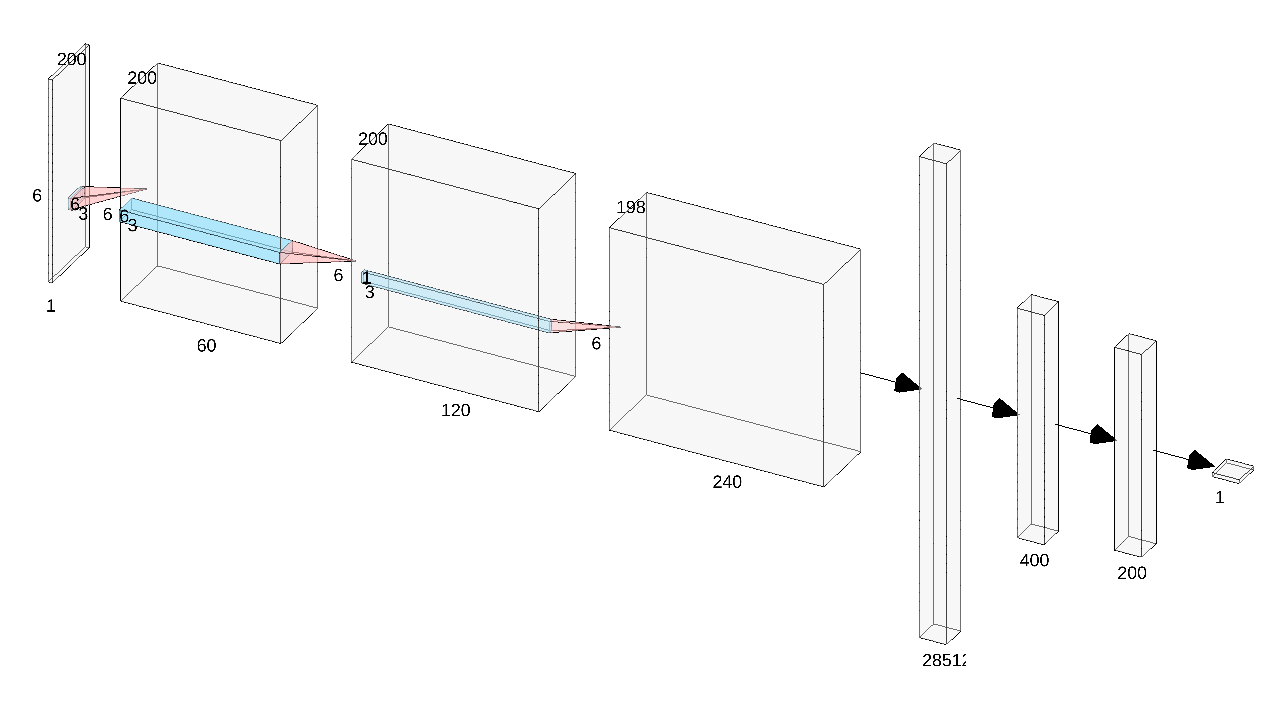
\includegraphics[width=0.75\textwidth]{img/speed_net.png}
   \caption{CNN architecture used for the speed regression task, adapted from \cite{DBLP:journals/corr/abs-1802-02209} (the dimensions of the blocks are not in scale).
   The input of this network is a window of IMU measurements, and the output corresponds to the speed (velocity norm) estimate for the time sample corresponding to the last time sample of this window.}
   \label{fig:speed_net}
\end{figure}

We make this design choice in order to reduce the number of parameters used by the architecture, as this number heavily depends on the size of the input IMU matrix $\mathbf{\hat{M}}$.
In fact, even after applying the pooling, the total number of trainable weights of the model is more than 18 million, where most of them come from the connection between the flattened convolutional feature vector and the first dense layer.

After some necessary pre-processing of the dataset which will be discussed next, the model is able to fit the training data accurately.
Unfortunately however, it is not able to successfully regress the drone speed on data from different validation sets (see Figure \ref{fig:speed_prediction_train_and_val}).
In fact, the training of this model took 150 epochs, at which point it was interrupted because the validation accuracy stopped improving.
We also left the model continue training, and eventually it could fit almost perfectly the training data around epoch 180, but no significant improvement would occur on the validation set.

\begin{figure}[h]
   \centering
   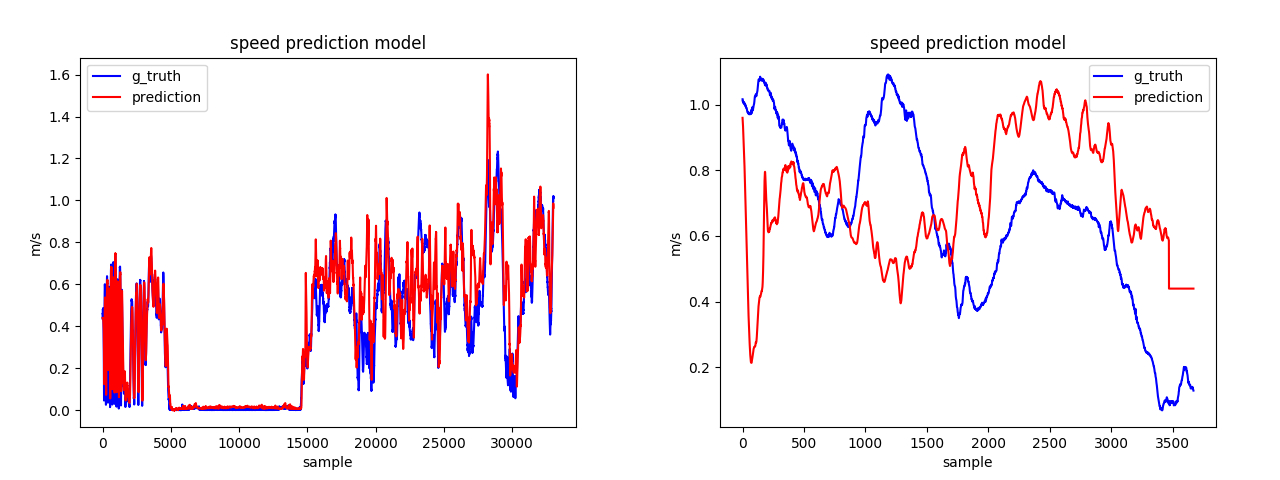
\includegraphics[width=0.90\textwidth]{thesis_template/img/speed_prediction_training_and_validation.jpg}
   \caption{Prediction of the speed regression model on the training (left) and testing (right) EuRoC dataset. Although the former prediction is accurate, it is clear that the model is failing for the validation set.}
   \label{fig:speed_prediction_train_and_val}
\end{figure}

Such fact leads us to the hypothesis that the model is heavily over-parametrized for the simplicity of its output, and it has in fact overfit a mapping between IMU readings and output speed in the training set. 
Moreover, as pointed out by \cite{DBLP:journals/corr/abs-1802-02209}, it should not be possible to fully predict the state $\mathbf{x}(k+w)$ or any of its sub-components, without having the initial state $\mathbf{x}(k)$. 
In other words, it should not be possible for the model to learn a reliable mapping $f_\theta\left(\mathbf{\hat{M}}_k\right)\mapsto\hat{s}(k)$ for any $\theta$, unless there was some encoding of the initial state somehow in the IMU readings that we are not aware of.
Therefore, whatever this CNN model was learning to regress the speed of the drone, it is most likely just an overfit of the training data.

To test this hypothesis, we use a synthesized version of the EuRoC dataset, where noise has been completely removed from the IMU.
In particular, we take a second flight sequence (not used in training), and generate \emph{ideal} IMU data with the package\href{https://github.com/zurich-eye/ze\_oss}{Zurich Eye VI simulator}.
Then, we make predictions with the model using this dataset, surprisingly obtaining not terrible results, as shown in Figure \ref{fig:speed_prediction_ideal_filtered}.
Even though the IMU has been completely removed of its noise, and this dataset is synthetic, this result points out that maybe there is something more to learn from the state in the IMU measurements.

\begin{figure}[h]
   \centering
   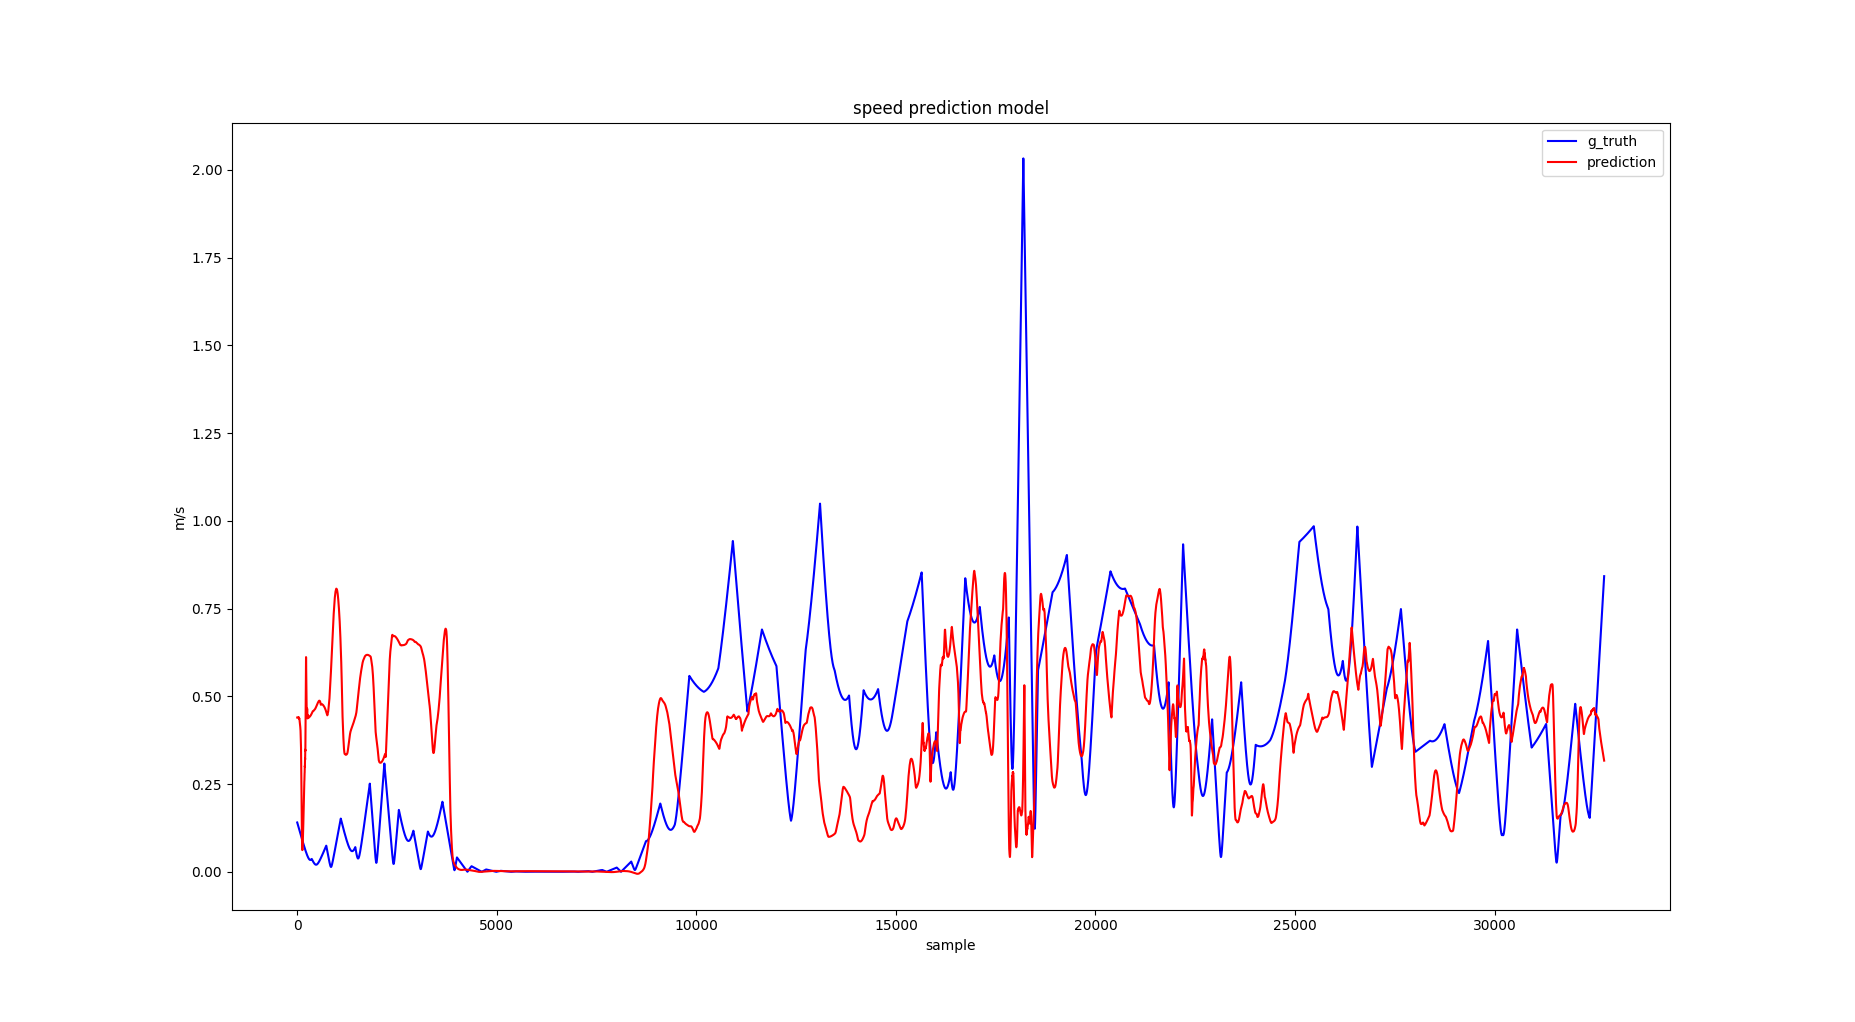
\includegraphics[width=0.85\textwidth]{thesis_template/img/ideal_filtered_speed_prediction_expandedplot.png}
   \caption{Predictions of the CNN speed regression model trained with filtered EuRoC data on a noiseless synthetic test dataset, generated from a difference sequence of the EuRoC dataset.}
   \label{fig:speed_prediction_ideal_filtered}
\end{figure}

To wrap up this first experiment, we emphasize two interesting conclusions we reach from the results:
\begin{itemize}
    \item In the original work \cite{DBLP:journals/corr/abs-1808-03485} that inspired this model, the main purpose of the authors is to train a deep regressor to provide a low-confidence speed prior for a recursive EKF pipeline, proposed in \cite{DBLP:journals/corr/SolinCRK17}. 
    We have argued why this kind of predictor will likely never be able to reliably learn a reliable encoding of the state from IMU measurements, and why the overall architecture of this model, with so many parameters, is not optimal. 
    However, as we will discuss in Section \ref{sec:pre_int_training}, it is indeed possible to learn a prior from $\mathbf{\hat{M}}_k$ that does not exactly represent the future state $\hat{s}(k)$, but can nevertheless be used to constrain it. 
    Furthermore, we have seen that, in an ideal test dataset, this model can still output a speed regression that somewhat makes sense. 
    Therefore, we leave as future work to incorporate this output, or maybe a more complex one (like a full velocity vector $\mathbf{\hat{v}}$), as an observation update to an EKF ogr similar state estimation algorithm.
    \item Despite that we will move on to a second kind of task in the incoming Section \ref{sec:imu_state_int}, we did gain some important knowledge with this first model and task about how to pre-process the inertial data, which we discuss in the appendix, in Section \ref{sec:euroc_filtering}.
\end{itemize}


\section{Second model: IMU state integrator}\label{sec:imu_state_int}

From the knowledge gathered during the previous model iteration, we set ourselves a new objective: train a model to perform noise-reduced IMU integration. 
In other words, we want to train a model that somehow learns to filter out the noise from $\mathbf{\hat{M}}_k$, and then use that to perform IMU integration.
In order to do this, we clearly learned in Section \ref{sec:speed_reg} that we require, besides the IMU data itself, to input the initial state $\mathbf{x}(k-w)$ to the model, as otherwise trying to predict $\mathbf{x}(k)$ is not mathematically feasible.
Put in equation form, for this task we want to train a deep regressor that performs the mapping \ref{eq:state_integration_problem}.
\begin{equation}\label{eq:state_integration_problem}
    f_\theta\left(\mathbf{x}(k-w),\mathbf{\hat{M}}_k\right)\mapsto\mathbf{\hat{x}}(k), \;\;\; \mathbf{x}(k)=\begin{pmatrix}\mathbf{p}\\ \mathbf{v}\\ \mathbf{q}\end{pmatrix}\in \mathbb{R}^{10}
\end{equation}
Where $\mathbf{p}, \mathbf{v}\in\mathbb{R}^3$ represent the $(x,y,z)$ position and velocity vectors in Euclidean space, and $\mathbf{q}\in\mathbb{Q}^4$ represents the unitary quaternion describing the rotation from the inertial frame $W$ to the body frame $B$. 
In other words, $\mathbf{q}$ is the unit quaternion form of the rotation matrix $\mathbf{R}_{W\!B}\in SO(3)$.
Notice that the members of the unitary rotation quaternion group $\mathbb{Q}^4$, although having 4 components, only three of them are independent.

To the best of our knowledge, this task had not been performed with a deep model in the literature yet in a 3-dimensional setup.
Consequently, we could not use any NN architecture as a foundation, so we designed our own model with the mathematical graph flow of IMU integration in mind.
Furthermore, since we verified that convolutional layers were indeed being able to generate a meaningful representation of $\mathbf{\hat{M}}_k$ in Section \ref{sec:speed_reg}, we used them once again to process the IMU data during the first layers of the model. 
The first architecture iteration for this task is shown in Figure \ref{fig:state_int_v0}.

\begin{figure}
    \centering
    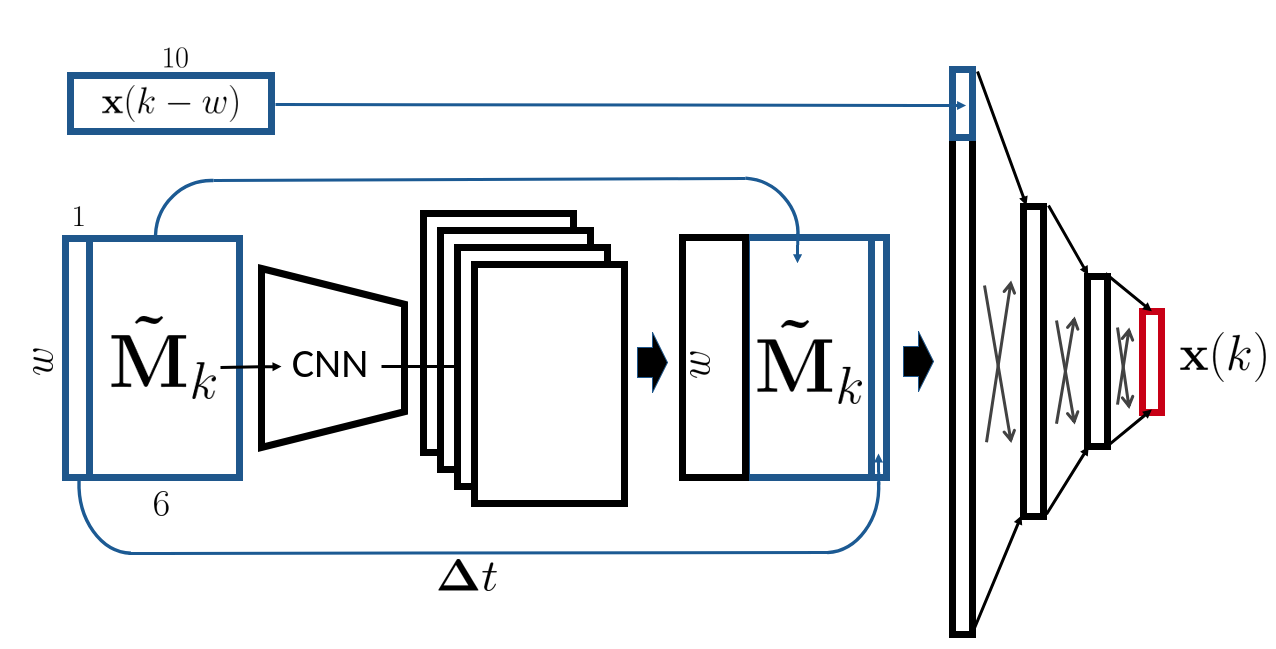
\includegraphics[width=\textwidth,height=\textheight,keepaspectratio]{thesis_template/img/imu_int_net.png} 
    \caption{Schematic architecture of IMU integration network. The IMU measurement matrix $\mathbf{\hat{M}}_k$ is processed by a series of convolutional layers, and the resulting generated feature vector is concatenated with the original $\mathbf{\hat{M}}_k$, and the $\Delta t$ vector, which contains the time difference between consecutive measurements.
    The concatenated tensor is then fed through one more convolutional layer, flattened, and appended to the initial state $x(k-w)$.
    Finally, three dense layers are applied, which output the predicted state $\mathbf{\hat{x}}(k)$}
    \label{fig:state_int_v0}
\end{figure}

The intuition behind the architecture is the following: with the convolutional block, we extract features from $\mathbf{\hat{M}}_k$. 
The convolution layers are designed so that gyroscope and accelerometer readings are not convolved together (by using the right kernel sizes and strides), as they physically represent different things. 
Also, besides using less channels than before in Figure \ref{fig:speed_net}, we add one extra convolutional layer that summarizes the channel dimension to only 5 components, to reduce the number of parameters needed for the final dense layers.
Then, this feature vector is concatenated with the original $\mathbf{\hat{M}}_k$ and the $\boldsymbol{\Delta}\mathbf{t}$ vector (which is a $w\times 1$ vector containing the time difference between two consecutive readings) and a final convolutional layer is applied.
The kernel of this layer is designed to occupy the entire length of the joint matrix, with the hope that it will learn to integrate the $\boldsymbol{\Delta} t$ into the system.

Finally, the resulting tensor is flattened, concatenated with the initial state, and fed into a sequence of Dense layers with ReLU activation, with the final layer outputting a 10-dimensional vector, as in \ref{eq:state_integration_problem}.
The last dense layer does not use any activation function. 
We decided to concatenate the convolutional feature vector with the original IMU matrix $\mathbf{\tilde{M}}_k$ for debugging purposes in later stages; i.e. to see whether the network was actually taking advantage of the convolutional layers.
This network has a total of 440K trainable parameters, and one epoch is trained in around 12 seconds in an i7 CPU. 

For this task, we investigate a second MAV dataset: MIT's BlackBird (BB) \cite{antonini2018blackbird}.
Compared to EuRoC dataset, the BB dataset has higher frequency ground truth annotations, more recorded sequences (a total of over 10h and 60km of data) and also more aggressive motion, with a top speed of up to 7m/s. 
By contrast, EuRoC reaches a top speed of 2.3m/s.

\subsection{First Iteration}
For the first iteration of this task, we train the model described in Figure \ref{fig:state_int_v0} with a smaller IMU window than last time: $w=50$. 
In the BB dataset, which uses an IMU that measures at 100Hz, this represents a 0.5s time interval.
The optimal parameters $\theta^*$ for this model are also recovered using the backpropagation algorithm with an Adam optimizer. 
The loss function chosen to be minimized during this training is defined by \ref{eq:q_state_loss}.
\begin{equation}\label{eq:q_state_loss}
    \mathcal{L}= \sum{\left \|\mathbf{p}-\mathbf{\hat{p}}  \right \|_2^2} + \sum{\left\|\mathbf{v}-\mathbf{\hat{v}}  \right \|_2^2} + \left |\sin\left(\left(\mathbf{q}^{-1}\mathbf{\hat{q}}\right)_\measuredangle \right)  \right |.
\end{equation}
Where $\mathbf{q}^{-1}\mathbf{\hat{q}}$ computes the quaternion that rotates $\mathbf{q}$ to $\mathbf{\hat{q}}$, and the operator $\measuredangle$ represents its angle.
The $|\sin(\cdot)|$ operation is then used to compensate for the periodicity of the angle error.

As a proof of concept, this model was trained on one of the easiest flights in the dataset: the flight sequence \emph{Thrice} (which barely has any motion in the z axis) and with a maximum speed of 2m/s.
However, to test better the model, it was validated on the sequence \emph{BentDice}, which is a flight sequence with a lot more of z displacement. 
Additionally, the predictions were compared with manual IMU double integration as a baseline.

The results of this experiment reveal that the model outperforms double integration for predicting the $\mathbf{v}$ vector, and the x and y components of the $\mathbf{p}$ vector.
On the other hand, it is not quite reaching this baseline for the z elevation coordinate, which was expected as the training dataset was flat, or the rotation term $\mathbf{q}$.
Figure \ref{fig:imu_int_50} depicts such results.
The horizontal axis corresponds to one sample of the test dataset; i.e., for each sample $k$ the input to both the model and the double integration algorithm is $(\mathbf{x}(k-w), \mathbf{\hat{M}}_k)$ and the optimal output to be obtained is the ground truth in blue, representing $\mathbf{x}(k)$.
\begin{figure}
    \centering
    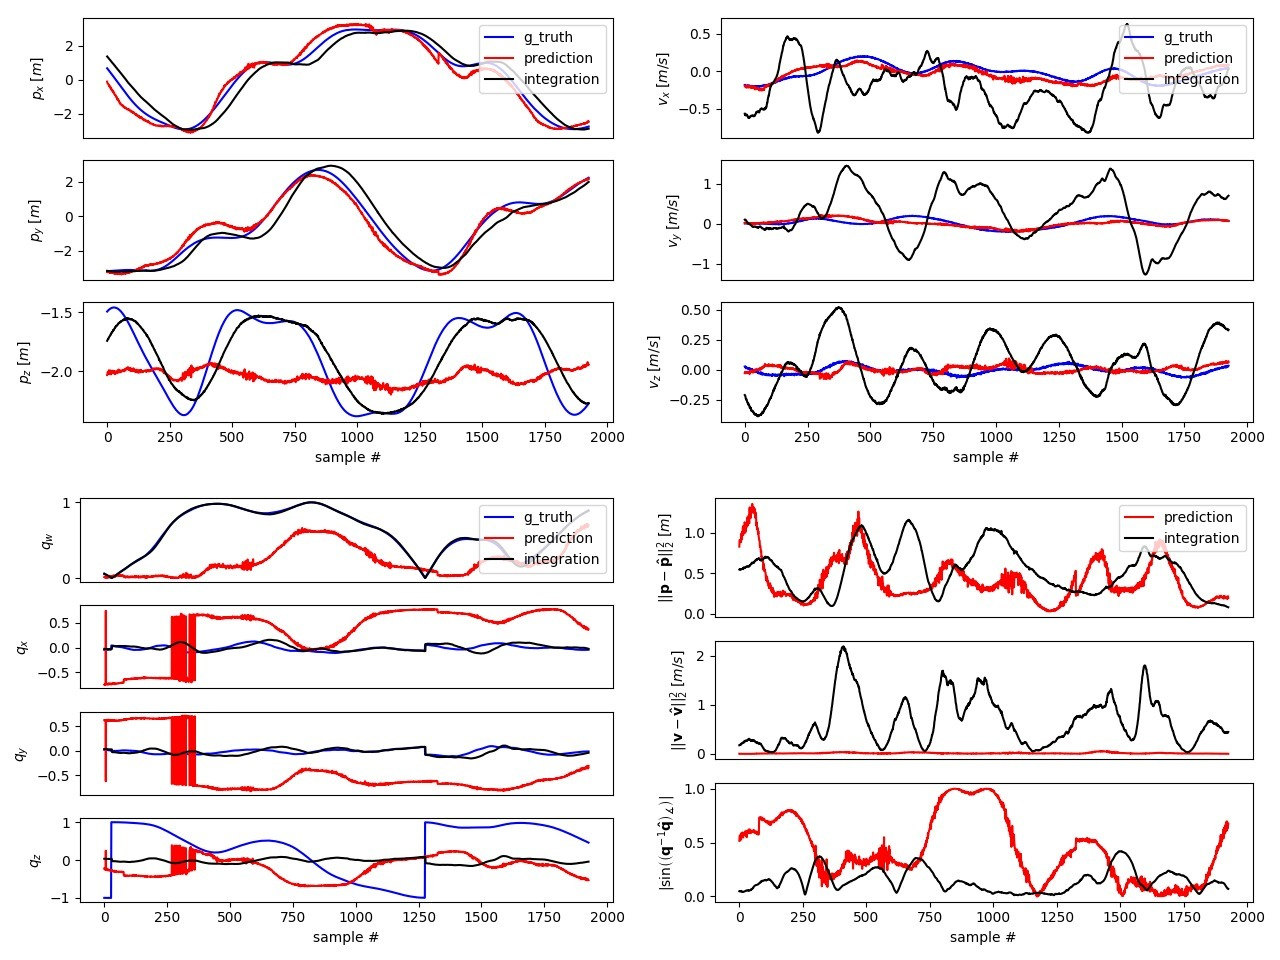
\includegraphics[width=\textwidth,height=\textheight,keepaspectratio]{thesis_template/img/imu_int_50.jpg} 
    \caption{Comparison between ground truth, model predictions and IMU double integration in set-aside validation set from the Blackbird \emph{bentDice}@2m/s sequence. For each x-axis entry, the inputs to the model and the double integration algorithm are the initial ground truth state $\mathbf{x}(k-w)$, and the output is the predicted state $\mathbf{x}(k)$. 
    The bottom right plot shows the error of both algorithms compared to the ground truth computed by the loss function \ref{eq:q_state_loss}.}
    \label{fig:imu_int_50}
\end{figure}

After inspection of this first test, we point out three main issues with this approach, for which we propose solutions in Sections \ref{sec:lie_algebra} and \ref{sec:pre_int_training}.
\begin{enumerate}
    \item \label{item:quaternion_loss_problem} The loss function \ref{eq:q_state_loss} for the rotation term is highly nonlinear, and the model cannot learn how to predict $\mathbf{q}$ properly. 
    This is probably because the constraint for the quaternion to be unitary creates nonlinear dependencies between the quaternion terms.
    In fact, the model showed to have serious problems even at fitting this distribution in the training set.
    \item \label{item:input_state_problem} Contradicting our own statement in the first paragraph of this section, the input state $\mathbf{x}(k-w)$ should \emph{not} be an input to the system.
    This is because if we feed $\mathbf{x}(k-w)$ to the deep model, and if the window of time corresponding to $w$ is small enough (in our case 0.5s), the model can learn an \emph{easy mapping} between $\mathbf{x}(k-w)$ and $\mathbf{x}(k)$ by not changing the input state.
    In other words, the initial state is necessary for performing IMU integration, but the model cannot rely on it to learn.
    \item Linked with problem \ref{item:input_state_problem}, in order to properly learn IMU integration in this setup it would be necessary to augment our dataset infinitely in order to make the model learn how to use the IMU data.
    This is because there are infinitely many initial and final position and velocity configurations.
\end{enumerate}

\subsection{Iteration 2: improved rotation loss term}\label{sec:lie_algebra}

In order to solve problem \ref{item:quaternion_loss_problem}, we draw inspiration from the approach proposed in \cite{DBLP:journals/corr/ClarkWWMT17} to enable a deep model to output in $SE(3)$ space (the general overview was discussed in Section \ref{sec:VIOnet}).
In the original work, the authors want to train a model to predict a series of homogeneous transformation matrices $\mathbf{T}$ from visual and inertial inputs. 
The definition of $\mathbf{T}$ is given by \ref{eq:homog_transf}. 
\begin{equation}\label{eq:homog_transf}
    _{W}\mathbf{T}_{AB}=\left\{\begin{pmatrix}_{W}\mathbf{R}_{AB}&_W\mathbf{t}_{AB}\\\mathbf{0}&1\end{pmatrix}\bigg\rvert\; _{W}\mathbf{R}_{AB}\in SO(3),\; _{W}\mathbf{t}_{AB}\in \mathbb{R}^3\right\}\in SE(3).
\end{equation}
Unfortunately, the special group $SO(3)$ is subject to orthogonality constraints, which are hard to figure out by a deep model.
This phenomenon is similar to what we are experimenting with the quaternion representation of rotation in $\mathbb{Q}^4$.

(\emph{All the algebra derivations that will follow are adaptations of chapter 8 of \cite{se3_tutorial}}).
On the other hand, the $SO(3)$ manifold is a subset of the invertible 
$3\!\times\!3$ matrices group $\mathbf{GL}(3, \mathbb{R})$. 
Any subgroup $G \in \mathbf{GL}(3, \mathbb{R})$ has two interesting properties:
\begin{enumerate}
    \item\label{item:G_linear_lie} $G$ is a linear Lie group.
    \item Derivable from property \ref{item:G_linear_lie}, the set $\mathfrak{g}$ in \ref{eq:lie_algebra_group}
    \begin{equation}\label{eq:lie_algebra_group}
    \mathfrak{g}=\left\{\mathbf{X}\in M (3,\mathbb{R})\rvert e^{t\mathbf{X}}\in G, \forall t \in \mathbb{R}\right\}.
    \end{equation}
    is a vector space tangent to $G$ at the identity $I$, and is closed under the Lie bracket operator, where $ M (3,\mathbb{R}):=\mathbb{R}^{3\!\times\! 3} \;\; s.t. \; \mathbf{GL}(3, \mathbb{R})\subset M (3,\mathbb{R})$.
\end{enumerate}

Effectively, this means that the matrix exponential operation $e^\mathbf{M}$, which has a convergent power series form denoted by \ref{eq:mat_power}, when $\mathbf{M}\in SO(3)$, computes its tangent vector space, which is an Euclidean space.
\begin{equation}\label{eq:mat_power}
    e^ M =\sum_{k=0}^{\infty }\frac{1}{k!} M ^k
\end{equation}
It so happens that the tangent space at of a Lie group $ M $ at its identity is also its lie algebra $\mathfrak{m}$ by definition.
Furthermore, there are two operations that relate the general Lie group $ M $ and its Lie algebra $\mathfrak{m}$:
\begin{itemize}
    \item The exponential map $\textrm{exp}:\mathfrak{m}\mapsto M $
    \item The logarithmic map $\textrm{log}: M \mapsto\mathfrak{m}$
\end{itemize}

For the case of the $SO(3)$ group, the corresponding Lie algebra is denoted by $\mathfrak{so}(3)$, and its base are three skew symmetric matrices corresponding to infinitesimal rotations along different axis.
Skew symmetric matrices in $\mathbb{R}^{3\!\times\!3}$ only have three independent components, and so can be perfectly mapped to a vector in $\mathbb{R}^3$ and \emph{vice versa} with the \emph{hat} $(\cdot)^{\wedge}$ and \emph{vee} $(\cdot)^{\vee}$ operators, as shown in \ref{eq:hat_and_vee}.
\begin{equation}\label{eq:hat_and_vee}
    \boldsymbol{\omega}=\begin{bmatrix}x\\y\\z\end{bmatrix}\rule{1cm}{0cm}\;
    \boldsymbol{\omega}^{\wedge}=\begin{pmatrix}0&-z&y\\z&0&-x\\-y&x&0\\\end{pmatrix}\rule{1cm}{0cm}\;
    ({\boldsymbol{\omega}}^\wedge)^\vee=\boldsymbol{\omega}.
\end{equation}
Finally, there are also specific exponential and logarithmic mappings that allow to map a rotation quaternion in $\mathbb{Q}^4$ to $\mathfrak{so}(3)$ and back, which have the forms \ref{eq:q_exp_map} and \ref{eq:q_log_map} respectively.
\begin{equation}\label{eq:q_exp_map}
    \mathbf{q}\doteq e_q^{\boldsymbol{\omega}}=\left\{ 
	\begin{array}{ll}
		(1,0,0,0)^\top  & \text{ , if }  \boldsymbol{\omega} = (0,0,0)^\top \\
		\left( \cos\dfrac{|\boldsymbol{\omega}|}{2}, \dfrac{\sin\dfrac{|\boldsymbol{\omega}|}{2}}{|\boldsymbol{\omega}|} ~ \boldsymbol{\omega} \right)^\top &  \text{ , otherwise}
	\end{array}
	\right.
\end{equation}
\begin{equation}\label{eq:q_log_map}
    \mathfrak{q}\doteq\boldsymbol{\omega}=\frac{2\arccos(q_r)}{|\mathbf{q}_v|}\mathbf{q}_v
\end{equation}

Recapitulating where we left off before this derivation, in \cite{DBLP:journals/corr/ClarkWWMT17} the authors want to train a model to output in $SE(3)$ space.
This was problematic because the $SO(3)$ rotation matrix in $SE(3)$ is subject to nonlinear constraints, which render any loss function to treat it very non-convex.
As a solution, they propose that the model predicts instead of the $SE(3)$ matrix, the Lie algebra representation of $\mathbf{T}$, whose rotation term in $\mathfrak{so}(3)$ can be expressed as a 3-component vector without any orthogonality constraints.
This makes the loss function significantly less nonlinear than when trying to work in $SO(3)$.

In our case, by adopting this idea, we train the deep model so it learns to predict the $\mathfrak{so}(3)$ representation of the rotation produced during a time sequence of length $w$.
This prediction is then manually remapped to $\mathbb{Q}^4$ with a final, non-trainable layer, in order to output a state with the same form as the initial state, as described in \ref{eq:state_integration_problem}. 
However, to simplify notation, we will state that the model now performs the mapping \ref{eq:state_integration_problem_so3}:
\begin{equation}\label{eq:state_integration_problem_so3}
    f_\theta\left(\mathbf{x}(k-w),\mathbf{\hat{M}}_k\right)\mapsto\mathbf{\hat{x}}(k), \;\;\;
    \mathbf{x}(k)=\begin{pmatrix}\mathbf{p}\\ \mathbf{v}\\ \mathbf{q}\end{pmatrix}\in \mathbb{R}^{10},\;\;
    \mathbf{\hat{x}}(k)=\begin{pmatrix}\mathbf{\hat{p}}\\ \mathbf{\hat{v}}\\ \mathfrak{\hat{q}}\end{pmatrix}\in \mathbb{R}^{9}
\end{equation}
And with this formulation, the new loss function becomes \ref{eq:state_so3_loss}, where the rotation term has changed with respect to \ref{eq:q_state_loss}.
\begin{equation}\label{eq:state_so3_loss}
    \mathcal{L}= \left \|\mathbf{p}-\mathbf{\hat{p}}  \right \|_2^2 + \left\|\mathbf{v}-\mathbf{\hat{v}}  \right \|_2^2 + \left\|\textrm{log}\left(\mathbf{q}\right)-\mathfrak{\hat{q}}\right\|_2^2.
\end{equation}
Where $\textrm{log}(\mathbf{q})$ is the $\mathfrak{so}(3)$ representation via the logarithmic mapping \ref{eq:q_log_map} of $\mathbf{q}$.

From the architecture point of view, the change in the rotation prediction type only affects to the final layer of the network model, which instead of having a 10 unit dense layer, now its 9 units, so that the new model now performs the mapping \ref{eq:state_integration_problem_so3}.

After applying these changes we train the model this time on the 3D sequence \emph{bentDice}, i.e. the one that we used for validation in the previous iteration of the model.
First, we check that with the new formulation, the model is indeed able to fit in the rotation quaternion, as now it does not have the extra imposed constraint of the rotation being unitary.
We set aside a segment of the \emph{bentDice} sequence, which was not used for training, and use it as validation set.
Figure \ref{fig:so3_rotation_fit} demonstrates that the model performs quite good on this experiment.
Even more interestingly, we can see how the model appears even to be adapting to the sign flips of the rotation axes in the left figure.
This is interesting albeit not ideal, as this is also a form of added difficulty that the model has to overcome to perform well on the task. 
We will tackle this issue too in the next section.
\begin{figure}
    \centering
    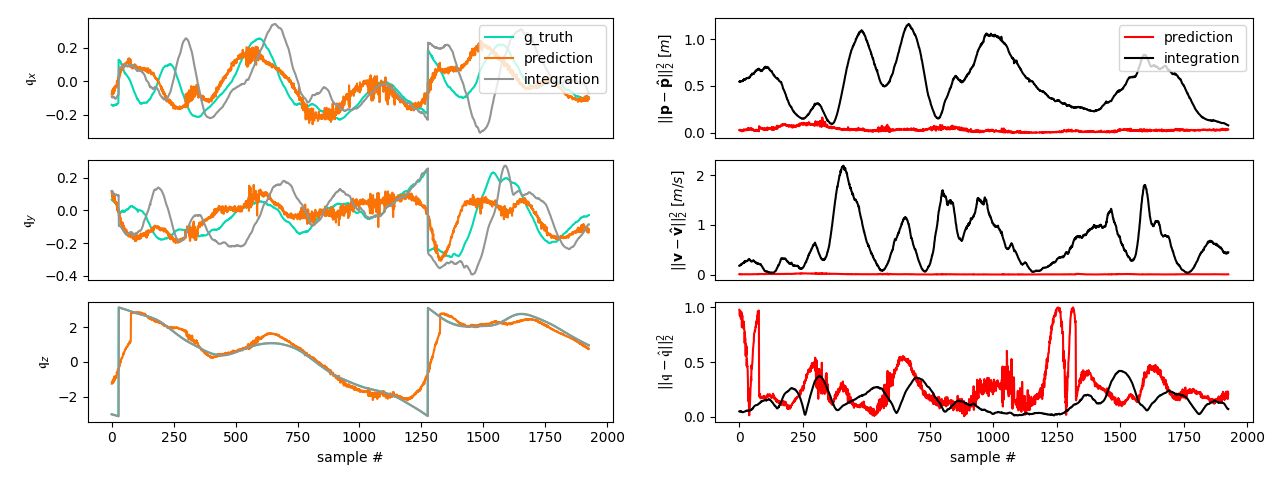
\includegraphics[width=\textwidth,height=\textheight,keepaspectratio]{thesis_template/img/imu_int_so3_rot_fit.jpg}
    \caption{Rotation predictions in Lie Algebra space in set-aside set from BB \emph{bentDice}@2m/s. The left plot shows the predictions of the three components of rotation state.
    The right are the losses (errors) for position, velocity and rotation for both the predicted and integrated states.
    The model is able to fit in the $\mathfrak{so}(3)$ rotation term, and this helps also to improve the position and velocity estimates, so that this model is constantly outperforming double-integration for the full state vector. }
    \label{fig:so3_rotation_fit}
\end{figure}

For the next experiment, we select a completely new validation dataset from the BB set, also rich in 3D motion, and also significantly more aggressive (with maximum speeds of 6m/s). 
We repeat the experiment, and summarize the results in Figure \ref{fig:so3_tiltedThrice_fit}.
Even though the predictions are good for $\mathbf{v}$ and for the $p_x$ and $p_y$, the model under-performs once again for the $\mathbf{q}$ term, and achieves a similar performance than integration for $p_z$. 
By closer inspection, it can be seen that this dataset is very rich in rotation axes sign flips, which is very likely to be the cause of the problem with the rotation fit, as we pointed out earlier. 
\begin{figure}
    \centering
    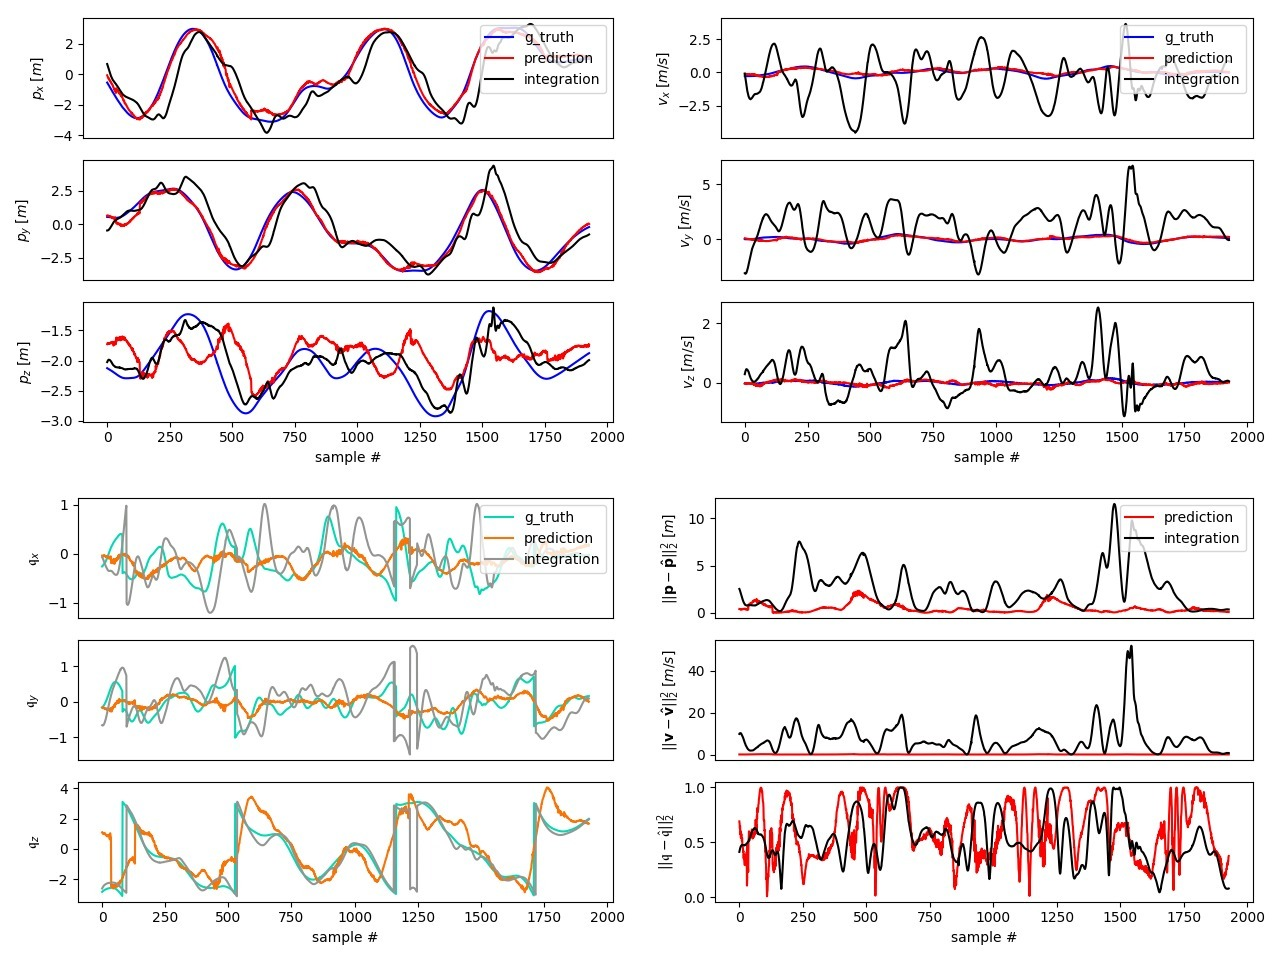
\includegraphics[width=\textwidth,height=\textheight,keepaspectratio]{thesis_template/img/imu_int_50_so3_tiltedThrice.jpg}
    \caption{Full comparison between ground truth, predicted and double-integrated states from IMU data. 
    The experiment is performed on the much more aggressive \emph{tiltedThrice}@6m/s BB sequence. 
    The bottom right plot again corresponds to the losses for the $\mathbf{p}$, $\mathbf{v}$ and $\mathfrak{q}$ terms, computed from \ref{eq:state_so3_loss}
    The model is unable to perform well the iterative task (right) on the training set
    $\mathbf{p}$ and $\mathbf{v}$ but both fail again in the rotation term.}
    \label{fig:so3_tiltedThrice_fit}
\end{figure}

For the final experiment round of this iteration, we set up a pipeline where the model prediction is fed back as input, together with the next sequence of IMU measurements, and repeat over a sequence of time. 
We refer to this test as the \emph{iterative} experiment in \ref{chap:experiments}. 
As a sanity check, this iterative experiment is first performed on the training dataset.
Unfortunately, despite that, the deep model is unable to successfully recover the trajectory using the iterative method, as shown in Figure \ref{fig:iterative_exp_fail}.
On the left plot, the 3D view of the predicted trajectory is plotted when the ground truth is fed to the model every $w$ time samples.
On the right, the model uses its own past prediction as new input in an iterative manner, every $w$ samples.
\begin{figure}
    \centering
    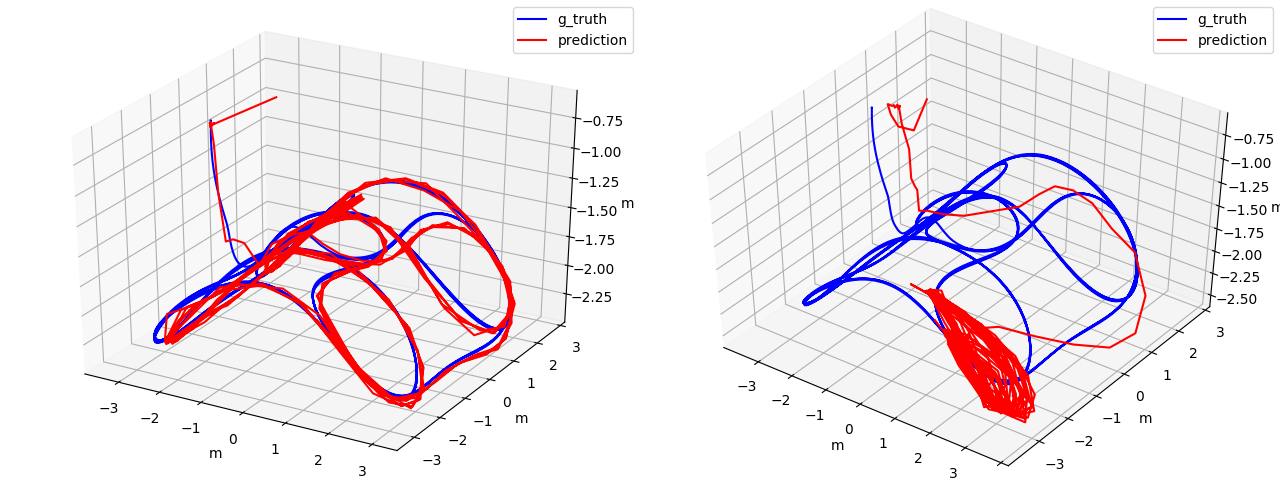
\includegraphics[width=\textwidth,height=\textheight,keepaspectratio]{thesis_template/img/iterative_exp_vs_gt.png}
    \caption{Left figure: prediction of the state integrator model on the training dataset. Right figure: prediction of the state integrator model on the training dataset, but only the first state is provided as input, instead of a state for every $\mathbf{\hat{M}}_k$.}
    \label{fig:iterative_exp_fail}
\end{figure}

This result yields to the conclusion that the model is too dependent on the initial state input of the system, and really is not learning IMU integration as well as originally thought. 
In section \ref{sec:exp_imu_int_so3} we perform a more in-depth analysis of what is going on, and conclude that, although the model learns some notion about integrating the IMU in the x and y axes, the architecture of this model is not optimal for learning this task.
We also conclude, however, than CNN layers are actually useful to process the IMU data.

In next section, we present a new approach to learn from inertial data for state integration in the next section, where the initial state is still fed to the model, but the model is prevented from learn from it.
The architecture that will be used implicitly enforces to learn the IMU integration task, while filtering the noise of the IMU at the same time.

\section{Third model: IMU pre-integration}\label{sec:pre_int_training}

As concluded in the literature review, feeding the initial state to the deep model is dangerous as it may up learning a mapping between initial state and final state.
Although in the experiments chapter we show that this is particularly not the main problem with the model proposed in Section \ref{sec:exp_imu_int_so3}, it is an issue worth finding a solution for.
This is especially the case when we use short values of $w$, as both input and output states will be similar.

To solve this, we draw inspiration once again from \cite{DBLP:journals/corr/abs-1802-02209}, which was discussed thoroughly in Section \ref{sec:ionet}.
In particular, in this work the authors train a deep model to predict 2D state increments, in the form $\Delta\mathbf{\hat{x}}=(\Delta\hat{l}, \Delta\hat{\psi})$, by demonstrating that it is possible to mathematically calculate these state increments just with the initial velocity, gravity vector, and IMU measurements (all of them in body frame).

We adopt the idea of calculating the state increments instead of the final state just from IMU data, as this will prevent over-fitting a mapping between initial and final states.
Furthermore, the span of the manifold of IMU data is arguably much more constrained than the span of the state vector.
In other words, it could be expected for the state position $\mathbf{p}$ to be arbitrarily large or small (as long as it is in $\mathbb{R}^3$), but the IMU data will likely never contain arbitrarily large angular speeds of accelerations, as it would not be feasible for the agent to move that fast.
This fact drastically reduces the amount of training examples this model would require to learn the task

We formulate a new problem setup in full 3D space by means of the work from Forster and his team, where they introduce the \emph{IMU pre-integration} theory for the first time \cite{DBLP:journals/corr/ForsterCDS15}.
We start by defining some notation:
\begin{enumerate}
    \item $\mathbf{R}_{WB}\mapsto \mathbf{R}\doteq$ rotation from world ($W$) frame to IMU ($B$) frame in $SO(3)$.
    \item\label{lab:w_frame} $_W\mathbf{x}\mapsto\mathbf{x} \doteq$ any vector in $\mathbb{R}^3$ with physical meaning defined in the $W$ reference frame.
    \item $\mathbf{x}_i\doteq$ a physical property (also in $W$ frame by means of point \ref{lab:w_frame}) measured at time index $i$.
    \item $\mathbf{\tilde{x}}\doteq$ observation of physical property (\emph{note}: we change the notation from $\mathbf{\hat{x}}$ to $\mathbf{\tilde{x}}$ to be consistent with \cite{DBLP:journals/corr/ForsterCDS15}).
    \item $\Delta\mathbf{x}_{ij}\doteq$ change of $\mathbf{x}$ between time indices $i$ and $j$, separated by a window $w$. We refer to $i$ and $j$ as the \emph{keyframe} indices.
    \item $\Delta\mathbf{\tilde{x}}_{ij}\doteq$ pre-integrated property between time indices $i$ and $j$ with IMU data.
\end{enumerate}
Furthermore, we will assume that the state of an agent at a specific time $i$ is given by the vector $(\mathbf{p}_i, \mathbf{v}_i, \mathbf{R}_i)^T$.
From vanilla IMU double integration, the final state given the initial state and IMU measurements is calculated by \ref{eq:imu_integration}:
\begin{eqnarray}\label{eq:imu_integration}
    \mathbf{R}_j & = & \mathbf{R}_i\prod_{k=i}^{j-1}\textrm{Exp}\left(\left(\tilde{\boldsymbol{\omega}}_k -\mathbf{b}^g_k - \boldsymbol\eta^g_k\right )\Delta t \right ) \nonumber\\
    \mathbf{v}_j & = & \mathbf{v}_i + \mathbf{g}\sum_{k=i}^{j-1}\Delta t + \sum_{k=i}^{j-1}\mathbf{R}_k\left(\tilde{\boldsymbol{a}}_k -\mathbf{b}^a_k - \boldsymbol\eta^a_k \right )\\
    \mathbf{p}_j & = & \mathbf{p}_i + \sum_{k=i}^{j-1}\left(\mathbf{v}_k\Delta t + \tfrac{1}{2}\mathbf{g}\Delta t^2 + \tfrac{1}{2}\mathbf{R}_k\left(\tilde{\boldsymbol{a}}_k -\mathbf{b}^a_k - \boldsymbol\eta^a_k \right)\Delta t^2\right)\nonumber
\end{eqnarray}
Where $\mathbf{b}^a_k$ and $\boldsymbol\eta^a_k$ are the bias and noise terms of the accelerometer $(a)$, and equivalently for the gyroscope $(g)$. We group all intermediate factors needed for integration in the variables $(\Delta\mathbf{R}_{ij},\Delta\mathbf{v}_{ij},\Delta\mathbf{p}_{ij})$, which exactly represent the state increment with the definitions \ref{eq:state_increments} (notice that $\mathbf{R}_i^T\mathbf{R}_k \doteq \Delta\mathbf{R}_{ik}$):
\begin{eqnarray}\label{eq:state_increments}
    \Delta\mathbf{R}_{ij} & = & \prod_{k=i}^{j-1}\textrm{Exp}\left(\left(\tilde{\boldsymbol{\omega}}_k -\mathbf{b}^g_k - \boldsymbol\eta^g_k\right )\Delta t \right )\nonumber\\
    \Delta\mathbf{v}_{ij} & = & \sum_{k=i}^{j-1}\mathbf{R}_i^T\mathbf{R}_k\left(\tilde{\boldsymbol{a}}_k -\mathbf{b}^a_k - \boldsymbol\eta^a_k \right )\Delta t\\
    \Delta\mathbf{p}_{ij} & = & \sum_{k=i}^{j-1}\left(\Delta\mathbf{v}_{ik}\Delta t +  \tfrac{1}{2}\mathbf{R}_i^T\mathbf{R}_k\left(\tilde{\boldsymbol{a}}_k -\mathbf{b}^a_k - \boldsymbol\eta^a_k \right)\Delta t^2\right)\nonumber
\end{eqnarray}
Such that \ref{eq:imu_integration} can be rewritten as \ref{eq:imu_integration_2}.
\begin{eqnarray}\label{eq:imu_integration_2}
    \mathbf{R}_j & = & \mathbf{R}_i\Delta\mathbf{R}_{ij}\nonumber \\
    \mathbf{v}_j & = & \mathbf{v}_i + \mathbf{g}\sum_{k=i}^{j-1}\Delta t + \mathbf{R}_i\Delta\mathbf{v}_{ij}\\
    \mathbf{p}_j & = & \mathbf{p}_i + \mathbf{v}_i\sum_{k=i}^{j-1}\Delta t +  \tfrac{1}{2}\mathbf{g}\Delta t^2 + \mathbf{R}_i\Delta\mathbf{p}_{ij} \nonumber
\end{eqnarray}
Notice that the equations in \ref{eq:state_increments} have the intermediate biases and noise terms $\mathbf{b}_k$ and $\boldsymbol{\eta}_k$ in their definitions.
In \cite{DBLP:journals/corr/ForsterCDS15}, it is assumed that the bias changes slow enough so that it remains constant between keyframes $i$ and $j$ (for that, the $w$ parameter can't be very large).
The noise terms are then isolated according to \ref{eq:pre_int_x}.
\begingroup
\setlength{\arraycolsep}{2pt} % Default value: 6pt
\renewcommand{\arraystretch}{1.8} % Default value: 1
\begin{eqnarray}
    \Delta\mathbf{R}_{ij} & = & \Delta\mathbf{\tilde{R}}_{ij}\textrm{Exp}\left(\delta\boldsymbol{\phi}_{ij}\right)
        \left\{
        \begin{array}{rll}
            \Delta\mathbf{\tilde{R}}_{ij} & \doteq  & \prod_{k=i}^{j-1}\textrm{Exp}\left(\left(\tilde{\boldsymbol{\omega}}_k -\mathbf{b}^g_k \right )\Delta t \right ) \\ 
            \delta\boldsymbol{\phi}_{ij} & \doteq  & \prod_{k=i}^{j-1}\boldsymbol\eta^g_k\Delta t
        \end{array}
        \right.
        \nonumber\\
    \Delta\mathbf{v}_{ij} & = & \Delta\mathbf{\tilde{v}}_{ij} - \delta\mathbf{v}_{ij}
        \left\{
        \begin{array}{rll}
            \Delta\mathbf{\tilde{v}}_{ij} & \doteq & \sum_{k=i}^{j-1}\Delta\mathbf{\tilde{R}}_{ik}\left(\tilde{\boldsymbol{a}}_k -\mathbf{b}^a_k\right )\Delta t\\
            -\delta\mathbf{v}_{ij} & \doteq & 
            \sum_{k=i}^{j-1}{f_{\delta\mathbf{v}}\left(\Delta\mathbf{\tilde{R}}_{ik}, \delta\boldsymbol{\phi}_{ik}, \tilde{\boldsymbol{a}}_k, \mathbf{b}^a_k\right)}
        \end{array}
        \right.
        \label{eq:pre_int_x}\\
    \Delta\mathbf{p}_{ij} & = & \Delta\mathbf{\tilde{p}}_{ij} - \delta\mathbf{p}_{ij}
    \left\{
        \begin{array}{rll}
            \Delta\mathbf{\tilde{p}}_{ij} & \doteq & \sum_{k=i}^{j-1}{\left(\tfrac{1}{2}\Delta\mathbf{\tilde{R}}_{ik}\left(\tilde{\boldsymbol{a}}_k -\mathbf{b}^a_k\right )\Delta t^2+\Delta\mathbf{\tilde{v}}_{ik}\Delta t\right)}\\
            -\delta\mathbf{p}_{ij} & \doteq & 
            \sum_{k=i}^{j-1}{f_{\delta\mathbf{p}}\left(\delta\mathbf{v}_{ik}, \Delta\mathbf{\tilde{R}}_{ik}, \delta\boldsymbol{\phi}_{ik}, \tilde{\boldsymbol{a}}_k, \mathbf{b}^a_k \right)}
        \end{array}
        \right.
        \nonumber
    \raisetag{20pt}
\end{eqnarray}
\endgroup
Where $f_{\delta\mathbf{v}}(\cdot)$ and $f_{\delta\mathbf{p}}(\cdot)$ are functions that calculate the error terms for a given time index $k$, whose full expression can be found in \cite{DBLP:journals/corr/ForsterCDS15}. 
We are omitting them here for readability reasons, since we won't use them in this work. 
Also, it can indeed be seen that the three pre-integration factors can be computed just from the IMU measurements, although they are dependent on each other. 
In other words, $\Delta\mathbf{\tilde{v}}_{ij}$ depends on $\Delta\mathbf{\tilde{R}}_{ij}$ and $\Delta\mathbf{\tilde{p}}_{ij}$ on $\Delta\mathbf{\tilde{v}}_{ij}$ and $\Delta\mathbf{\tilde{R}}_{ij}$.

Next, we can substitute back the left-hand sides of \ref{eq:pre_int_x} into \ref{eq:imu_integration_2} and isolate the pre-integration terms, such that we obtain an equivalent way of computing them from the ground truth.
In this scenario, we can assume that there will be no noise terms:
\begin{eqnarray}\label{eq:gt_pre_integration}
    \Delta\mathbf{\tilde{R}}_{ij} & = & \mathbf{R}_i^T\mathbf{R}_j\cancelto{1}{\textrm{Exp}\left(\delta\boldsymbol{\phi}_{ij}\right)} = \Delta\mathbf{R}_{ij}\nonumber\\
    \Delta\mathbf{\tilde{v}}_{ij} & = & \mathbf{R}_i^T\left(\mathbf{v}_j - \mathbf{v}_i - \mathbf{g}\sum_{k=i}^{j-1}\Delta t\right) + \cancelto{0}{\delta\mathbf{v}_{ij}}= \Delta\mathbf{v}_{ij}\\
    \Delta\mathbf{\tilde{p}}_{ij} & = & \mathbf{R}_i^T\left(\mathbf{p}_j - \mathbf{p}_i - \mathbf{v}_i\sum_{k=i}^{j-1}\Delta t - \frac{1}{2}\mathbf{g}_i\sum_{k=i}^{j-1}\Delta t^2\right) + \cancelto{0}{\delta\mathbf{p}_{ij}}= \Delta\mathbf{p}_{ij}\nonumber
\end{eqnarray}

In other words, we can train a model to learn to predict the state pre-integration variables $(\Delta\mathbf{\tilde{R}}_{ij},\Delta\mathbf{\tilde{v}}_{ij},\Delta\mathbf{\tilde{p}}_{ij})^T$ just from the IMU data $\mathbf{\tilde{M}}_k$.
The exact values for these variables for training can be obtained via \ref{eq:gt_pre_integration},
which we can compute from the state ground truth data.
Then, the predictions for $(\Delta\mathbf{\tilde{R}}_{ij},\Delta\mathbf{\tilde{v}}_{ij},\Delta\mathbf{\tilde{p}}_{ij})^T$ can be used in a non-trainable way to output the actual final state using \ref{eq:imu_integration_2}, given the input state $(\mathbf{R}_i, \mathbf{v}_i, \mathbf{p}_i)^T$.
With this strategy, we ensure that the initial state is not used for the model to over-fit a mapping to the output state.
Also, since the ground truth data for the pre-integration factors is computed without the noise terms, the model will be forced to learn a way to filter out these from the IMU measurements.

Finally, we can combine the current pre-integration idea, with the $\mathfrak{so}(3)$ rotation training derived in Section \ref{sec:lie_algebra}, which we found helps to fit the rotation state. 
Furthermore, we study yet another interesting training approach from the same publication \cite{DBLP:journals/corr/ClarkWWMT17}, where a set of two loss functions is used.
While the first loss group is computed from the prediction error at the state increment level $\Delta \mathbf{x}^e$, the second uses the prediction error at the state output level.
According to the authors, the state increment loss layer helps the model converge to the right structure to perform IMU integration during the earlier epochs, while the second helps it fine-tune to the output at later stages. 
This one, and other different training strategies for this model will be compared in the experiments section.

\subsubsection{Pre-integration model overview}

Let us structure and formalize all the information above. 
Our \emph{pre-integration model} is in fact composed of two concatenated sub-models $f_\theta$ and $g$, where only the former is trainable.
They respectively perform the mappings \ref{eq:pre_integration_model}.
\begin{IEEEeqnarray}{rlll}\label{eq:pre_integration_model}
    f_\theta\!\left(\mathbf{\tilde{M}}_k\right) \;&\; \mapsto \;&\; \Delta\mathbf{\tilde{x}}_{ik'}, \;&\; \forall k' \in \{i,i+1,...,j-1\}.\nonumber\\
    g\!\left(\left.\!\!\Delta\mathbf{\tilde{x}}_{ik'}\right\rvert_{k'=j-1}, \mathbf{x}(k-w)\right)\;&\; \mapsto \;&\; \mathbf{x}(k). \;&\; \\
    h_\theta\left(\left.\mathbf{\tilde{M}}_k\right\rvert\mathbf{x}(k-w)\right) \;&\; \mapsto \;&\; \mathbf{x}(k), \;&\; h_\theta \doteq g \circ f_\theta\nonumber.
\end{IEEEeqnarray}
Recall that $\mathbf{\tilde{M}}_k$ contains all the IMU measurements from $k-w$ to $k$ (see definition \ref{eq:imu_img}) and $\Delta\mathbf{\tilde{x}}_{ik}$ are the pre-integrated states \ref{eq:gt_pre_integration}, but with the rotation term is in $\mathfrak{so}(3)$ (\ref{eq:recall_deltax}).
\begin{IEEEeqnarray}{rllll}\label{eq:recall_deltax}
    \Delta\mathbf{\tilde{x}}_{ik} \;&\; \doteq \;&\;     \begin{pmatrix}\Delta\mathfrak{\tilde{q}}_{ik}\\\Delta\mathbf{\tilde{v}}_{ik}\\\Delta\mathbf{\tilde{p}}_{ik}\end{pmatrix} \;&\; s.t. \;&\; \Delta\mathfrak{\tilde{q}}_{ik} \in \mathbb{R}^{w\times3} , \Delta\mathbf{\tilde{v}}_{ik} \in \mathbb{R}^{w\times3} , \Delta\mathbf{\tilde{p}}_{ik} \in \mathbb{R}^{w\times3}. \nonumber\\
    \mathbf{x}(k) \;&\; \doteq \;&\; \begin{pmatrix}\mathbf{\tilde{p}}(k)\\\mathbf{\tilde{v}}(k)\\\mathbf{\tilde{q}}(k)\end{pmatrix} \;&\; s.t. \;&\; \mathbf{\tilde{p}}(k)\in\mathbb{R}^{3}, \mathbf{\tilde{v}}(k)\in\mathbb{R}^{3}, \mathbf{\tilde{q}}(k)\in\mathbb{R}^{4}.
\end{IEEEeqnarray}
Note that the $g$ function in \ref{eq:pre_integration_model} must perform first the exponential mapping from $\mathfrak{so}(3)$ to $\mathbb{Q}^4$ and then apply \ref{eq:imu_integration_2} to integrate the state.
More importantly, all these operations must be implemented in a differentiable way, so that the back-propagation algorithm can pass the losses through this last layer throughout the entire joint model $h_\theta$\footnote{To operate with quaternions in Tensorflow2.0a in a differentiable way, we adapt the existing Python library https://github.com/PhilJd/tf-quaternion}.

Likewise, and using the two-fold loss concept from \cite{DBLP:journals/corr/ClarkWWMT17} introduced at the end of last section, $h_\theta$ has four different loss functions, one for each output.
The first three are simply the MSE of the predicted pre-integrated tensors with respect to the ones calculated from the ground truth. 
With a slight abuse of notation, we define the predicted values by the model to be denoted by the exponent $p$.
In this case, the loss functions for the pre-integrated outputs can be described as in \ref{eq:pre_int_loss}.
\begin{eqnarray}\label{eq:pre_int_loss}
    \mathcal{L}_{\Delta\mathbf{\tilde{x}}} & = & \mathcal{L}^e_{\mathbf{\mathfrak{q}}}+\mathcal{L}^e_\mathbf{v}+\mathcal{L}^e_\mathfrak{p} \nonumber\\
    & = & \sum{\left\|\textrm{log}\left(\Delta\mathbf{\tilde{q}}_{ik}\right)-\Delta\mathbf{\mathfrak{\tilde{q}}}^p_{ik}\right\|_2^2} + 
    \sum{\left\|\Delta\mathbf{\tilde{v}}_{ik}-\Delta\mathbf{\tilde{v}}^p_{ik}\right\|_2^2} +  \\
    & & + \sum{\left\|\Delta\mathbf{\tilde{p}}_{ik}-\Delta\mathbf{\tilde{p}}^p_{ik}\right\|_2^2} \;\;\; \forall k \in \{i, i+1, ..., j-1\} \nonumber
\end{eqnarray}
However, for the fourth loss for the state output $\mathcal{L}_\mathbf{x}$, we cannot use again the loss $\mathbb{R}^{10}$ \emph{state loss} defined in \ref{eq:q_state_loss}, as we saw that it disrupts the training of the rotation terms.
However, in our case, since the model is locked between the pre-integrated variables and the output state, adding this fourth loss is equivalent to increasing the weight of the last rows of these losses.
The total loss is simply a weighted sum of both (\ref{eq:combined_4_loss}):
\begin{equation}\label{eq:combined_4_loss}
    \mathcal{L}_T=a\mathcal{L}_{\Delta\mathbf{\tilde{x}}} + b\mathcal{L}_\mathbf{x}.
\end{equation}

We will also studying how $a$ and $b$ affect to the training process.

Before getting into details with the proposed architecture of this network, we summarize the advantages of this novel approach for deep IMU integration.
\begin{itemize}
    \item The relationship between state input and output does not directly affect the training of the model, and thus it is not possible for it to learn a trivial mapping between both.
    \item The pre-integrated rotation term is computed in Lie algebra, which suffers less nonlinearities than quaternion and allows to use standard L2 norm.
    \item The structure of the training graph can enforce the model to learn specific temporal dependencies between the different variables that mimic how IMU integration works.
    If the model is capable of learning integration even with this rigid structure, then the risk of overfitting is significantly lower.
    \item The training is based on state \emph{pseudo}-increments (i.e. IMU pre-integration). 
    This means that by using a moderately small window length hyperparameter $w$, we allow the rotation changes to be small enough so the training data does not suffer from sign flips, which are highly nonlinear and disturb training.
    \item The model has up to 4 different sources of loss, diminishing the problem of vanishing gradients.
    This allows safer usage of deeper architectures, as well as recurrent layers, which tend to suffer the most from vanishing gradients.
\end{itemize}
And, by contrast, the two main possible disadvantages of this approach:
\begin{itemize}
    \item The rigidity and inter-dependencies of the structure means that the model has to learn the integration task of the three states (position, velocity and rotation) with good quality. 
    Otherwise the result will be poor, as mistakes in the rotation and/or velocity pre-integrated values will affect also position.
    \item Because of all of the above, the training of this model will be challenging.
    
\end{itemize}

\subsubsection{Pre-integration model architecture}

With this setup in mind, we iterate on a new batch of models with the common structure shown in Figure \ref{fig:basic_pre_integration_model}

\begin{figure}[h]
   \centering
   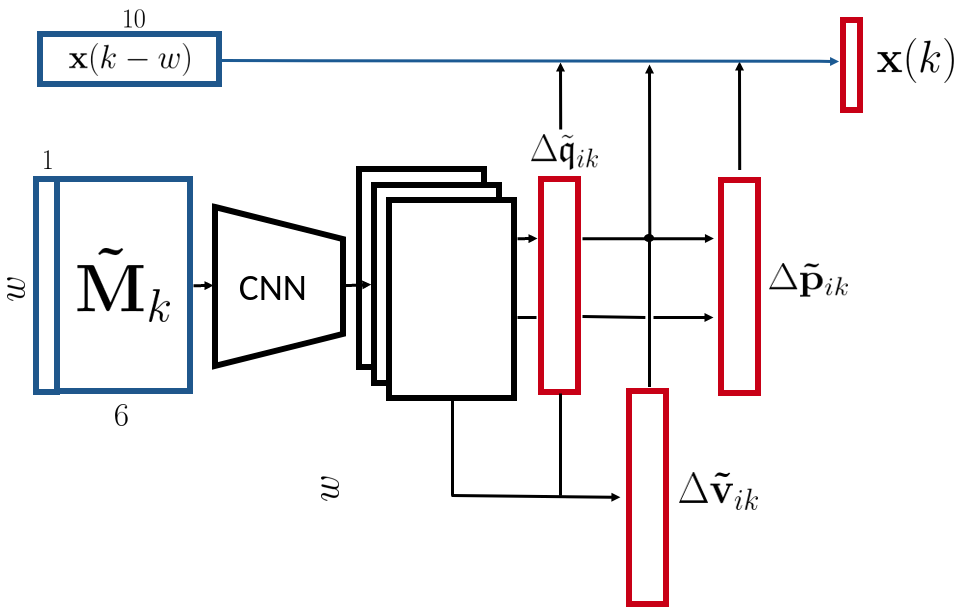
\includegraphics[width=0.75\textwidth]{img/imu_preintegration_general_net.png}
   \caption{Basic concept of the pre-integration network. Outputs in red, inputs in blue. The $\mathbf{\hat{M}}_k$ is processed by a convolutional block to generate a multidimensional feature vector.
   This vector is then used to compute the pre-integrated rotation term $\Delta\mathfrak{\tilde{q}}_{ik}$, which at its turn is used to compute the pre-integrated velocity matrix $\Delta\mathbf{\tilde{v}}_{ik}$.
   Finally, both these variables, plus the feature vector are combined to predict the final pre-integrated position $\Delta\mathbf{\tilde{p}}_{ik}$. 
   The state update is done by applying equations \ref{eq:imu_integration_2}.}
   \label{fig:basic_pre_integration_model}
\end{figure}

The main intuition behind the model is the following:
Once again, a series of convolution layers process the IMU input $\mathbf{\tilde{M}}_k$ and generate a feature vector. 
This feature vector is then used to output the first the pre-integration factor $\Delta\mathfrak{\tilde{q}}_{ik}$, corresponding to the rotation state. 
The model outputs this first, as it is the only one of the three that that can be computed on its own.
Then, both the convolutional feature vector and the pre-integrated rotation tensor are concatenated along the $w$ dimension, and used in a similar way to generate the $\Delta\mathbf{\tilde{v}}_{ik}$ term.
Finally, the feature vector and both pre-integration terms for rotation and velocity are concatenated, once again, along the $w$ dimension.
The resulting tensor is finally used by the model to generate the final pre-integration sequential term for position, $\Delta\mathbf{\tilde{p}}_{ik}$.

The current task is a challenging one, as it is supposed to mimic a very structured mathematical pipeline; the IMU double integration, but with the added twist of the pre-integrating factors.
Furthermore, one of the main aims of this final model is to be implementable real time in an hypothetical VIO platform, for which reason it is also important to keep the number of trainable parameters as low as possible.
Several iterations of fine-tuning of the model lead to the following refinements:

\textbf{Convolutional feature extractor}: For this module we leverage Temporal Convolutional Networks (TCN's) as the main building block.
This kind of CNN structure uses small dilated convolutional kernels with the same stride as the dilation rate, with the aim of rapidly expanding the receptive field of each neuron in the tensor channels \cite{DBLP:journals/corr/abs-1811-10166}.
Typically, a dilation and stride of 2 are used, so basically at layer $i$ a neuron has a receptive field of $2^i$. 

Furthermore, in order to extract both local and general features about the IMU matrix $\mathbf{\tilde{M}}_k$ we combine the TCN concept with the idea of an \emph{hourglass} structure.
This architecture was firstly introduced for the task of Human pose estimation in RGB images, achieving state-of-the-art accuracy outcomes \cite{DBLP:journals/corr/NewellYD16}.
It has proven to be efficient both at multi-scale feature extraction of spatially-correlated data and at keeping gradients alive using skip connections even with relatively deep models \cite{DBLP:journals/corr/PavlakosZDD16}.
Thanks to the extra receptive field expansion of TCN layers (which replace the traditional CNN in the hourglass), the global information can be condensed much faster, in which case we only use two recursive down-scalings of the input tensor in the hourglass module.

Something that we take extra care of, is to use reflection padding on the convolution kernels, since we don't want the information at the edges of the feature vector to be distorted by zero paddings.
Finally, the gyroscope and the accelerometer data are split and fed into to two separate hourglass modules, as it should not make any physical sense to process this data together.

\textbf{Pre-integration generator module}: the three pre-integrated variables to be generated $(\Delta\mathfrak{\tilde{q}}_{ik}, \Delta\mathbf{\tilde{v}}_{ik}, \Delta\mathbf{\tilde{p}}_{ik})$ are temporally very self-correlated. 
As such, we recycle the idea from the visual-inertial CNN-RNN architecture \cite{DBLP:journals/corr/ClarkWWMT17}, where an RNN layer (and in particular an LSTM) is exploited for this generative task (as we discussed in Section \ref{sec:VIOnet}). 
In their publication, the authors argue that using two layers of bidirectional LSTM's to generate temporally correlated data provides the best results compared to unidirectional or single-layered counterparts. 
We will not adopt any of the two ideas for different reasons:
\begin{itemize}
    \item Using bidirectional layers means that we break the very delicate alignment between the three variables in the pre-integration equations \ref{eq:pre_int_x}.
    In other words, for instance $\Delta\mathbf{\tilde{v}}_{ik}$ should only depend on $\Delta\mathfrak{\tilde{q}}_{ik'}$ for $k \in \{i, i+1, ..., i+k\}, \; k \leq w$. 
    \item Recurrent networks dramatically increase the inference time of the model, as these have to be processed sequentially.
    Since we will be needing already three recurrent layers (one for each pre-integration variable), we cannot afford stacking a second one on top.
\end{itemize}
However, we do adopt the idea of using a recurrent layer for generating these three outputs. 
In fact, empirical tests comparing GRU's \cite{DBLP:journals/corr/ChoMGBSB14} and LSTM revealed that the former outperforms both in training time and loss, so we chose it instead of LSTM.

\textbf{Pre-integrated variables: information passing}
One of the aims of this architecture and training setup is that we want to enforce the model to learn very precise temporal relationships between the variables that mimic equations \ref{eq:pre_int_x}.
As such, we implement the following constraints on $f_\theta$:
\begin{itemize}
    \item The GRU that generates $\Delta\mathfrak{\tilde{q}}_{ik'}$ will only use the TCN feature vector from the gyroscope.
    \item The output of a pre-integrated variable is passed to the next via a customly designed dense layer, that removes all connections to \emph{future} neurons. 
    E.g. $\Delta\mathfrak{\tilde{q}}_{ik'}$ can only be connected to $\Delta\mathbf{\tilde{v}}_{ik}$ for $k' \in \{i, i+1, ..., i+k\}, \; k \leq w$
    \item We don't use neither data or batch normalization between layers, as this model is very dependent on the scale of the input data.
\end{itemize}

The model with all of its refinements has a total of less than 180K trainable parameters, which is the lowest compared with the 440K of the second model, or the 18M of the first.
The overall structure is represented in Figure \ref{fig:full_pre_integration_model}, where represented by blue boxes, and outputs in red boxes.
Additionally, GRU cells are in green, untrainable connections in gray, and special, temporal aware dense connections in red.

\begin{figure}[h]
   \centering
   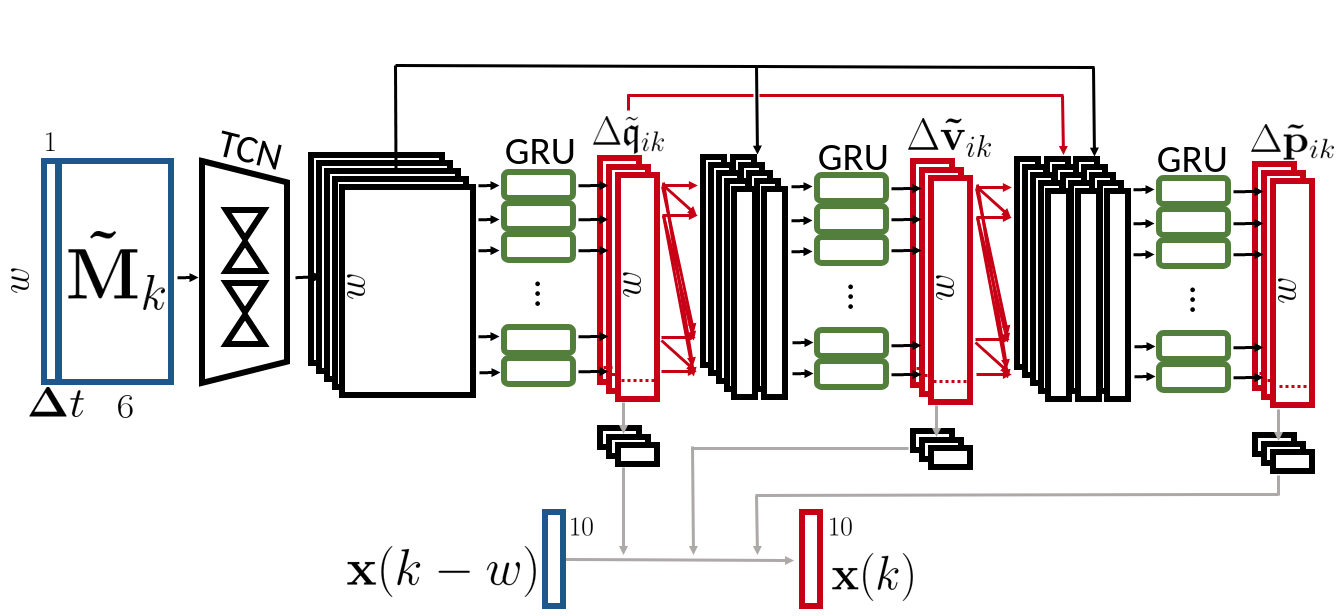
\includegraphics[width=0.95\textwidth]{thesis_template/img/pre_integration_full.png}
   \caption{Refined pre-integration network. Outputs in red, inputs in blue. Customized connections as red lines. Non-trainable connections as gray lines.
   The convolutional block is substituted by a recursive hourglass convolutional architecture with TCN layers.
   The layers that generate the pre-integrated variables are GRU units, and the custom connections ensure that variables can only depend on samples from the past and not the future, along the $w$ dimension.}
   \label{fig:full_pre_integration_model}
\end{figure}

In Chapter \ref{chap:experiments}, we will discuss our different attempts at training this model.